\documentclass[conference]{IEEEtran}

% ==============================
% PAQUETES
% ==============================
\usepackage[spanish]{babel}
\usepackage[utf8]{inputenc}
\usepackage[T1]{fontenc}
\usepackage{amsmath,amssymb}
\usepackage{graphicx}
\usepackage{cite}
\usepackage{url}
\usepackage{hyperref}
\usepackage{float}
\usepackage{booktabs}    % tablas IEEE más limpias
\usepackage{siunitx}     % unidades (dBm, MHz) opcional
\usepackage{tabularx}    % tablas que se ajustan a una columna

% ==============================
% DATOS DEL ARTÍCULO
% ==============================
\title{Sistema de Comunicaciones LoRa/APRS:\\
Definición de Alcance, Fundamentación Teórica y Marco Regulatorio en Costa Rica}

\author{
\IEEEauthorblockN{
Randy Fernández Aguilar \IEEEauthorrefmark{},
y
Luis Diego García Rojas  \IEEEauthorrefmark{} }
\vspace{2mm}
\IEEEauthorblockA{\IEEEauthorrefmark{}Escuela de Ingeniería Electrónica,
Instituto Tecnológico de Costa Rica (ITCR), 30101 Cartago, Costa Rica}
}

\begin{document}

\maketitle

% ==============================
% RESUMEN
% ==============================
\begin{abstract}
Este documento presenta el alcance y la investigación inicial para el desarrollo de un sistema de comunicaciones basado en tecnologías LoRa y APRS. Se establece la fundamentación teórica, arquitectura del sistema, parámetros físicos de operación y el análisis de la legislación costarricense aplicable.
\end{abstract}

\begin{IEEEkeywords}
LoRa, APRS, LPWAN, Comunicaciones Inalámbricas, Regulación del Espectro, Costa Rica.
\end{IEEEkeywords}

% ==============================
\section{Objetivos}

\subsection{Objetivo General}

Desarrollar el firmware de un iGate APRS basado en tecnología LoRa capaz de recibir paquetes de radio provenientes de nodos remotos y retransmitirlos hacia la red APRS-IS mediante conexión a Internet, cumpliendo con las condiciones técnicas y regulatorias establecidas para el uso del espectro en Costa Rica.
\subsection{Objetivos Específicos}

\begin{itemize}

\item Investigar los fundamentos teóricos de los sistemas de comunicación APRS y de la tecnología LoRa, incluyendo su arquitectura de red y parámetros físicos de operación.

\item Analizar la normativa costarricense relacionada con el uso del espectro radioeléctrico, con el fin de identificar las bandas de operación permitidas y sus restricciones técnicas.

\item Implementar un firmware capaz de recibir tramas LoRa provenientes de nodos remotos, procesarlas y reenviarlas hacia un servidor APRS mediante conexión a Internet.

\end{itemize}
% ==============================
\section{Introducción}

El crecimiento de aplicaciones de telemetría y monitoreo remoto ha impulsado el desarrollo de tecnologías de comunicación inalámbrica capaces de operar a largas distancias con bajo consumo energético. Entre estas tecnologías destaca LoRa (Long Range), una modulación basada en Chirp Spread Spectrum diseñada para redes de área amplia de baja potencia (LPWAN). Por otra parte, el sistema Automatic Packet Reporting System (APRS) es ampliamente utilizado en el servicio de radioaficionados para transmitir información digital como posición geográfica, mensajes cortos y datos de sensores en tiempo real.

La integración de tecnologías LoRa con la infraestructura APRS permite extender las capacidades de monitoreo y telemetría a largas distancias utilizando dispositivos embebidos de bajo consumo. El \textit{iGate}  cumple un rol fundamental dentro de la red APRS, ya que permite recibir paquetes transmitidos por radio y reenviarlos hacia la red global APRS-IS mediante conexión a Internet.

El informe se centrara en el desarrollo  e investigación de un firmware para un iGate APRS basado en tecnología LoRa, capaz de recibir tramas provenientes de nodos remotos y reenviarlas a la red APRS-IS. Este firmware permitirá validar la integración entre comunicaciones de radio de largo alcance y plataformas de visualización en línea.





\section{Fundamentación Teórica}

\subsection{APRS (Automatic Packet Reporting System)}

El Automatic Packet Reporting System (APRS) es un sistema digital de comunicación utilizado en el servicio de radioaficionados que permite el intercambio en tiempo real de información como posición geográfica, mensajes cortos, telemetría, datos meteorológicos y estado de estaciones \cite{aprs_web}. Fue desarrollado por Bob Bruninga, WB4APR, y opera principalmente sobre redes VHF utilizando el protocolo AX.25 para la transmisión de paquetes digitales.

Entre las principales aplicaciones del sistema APRS se encuentran:
\begin{itemize}
    \item Rastreo de vehículos y estaciones móviles mediante GPS.
    \item Monitoreo meteorológico en tiempo real.
    \item Comunicación de mensajes cortos entre radioaficionados.
    \item Coordinación en situaciones de emergencia.
    \item Telemetría de sensores remotos.
\end{itemize}

APRS utiliza principalmente el protocolo AX.25 para la transmisión de tramas digitales sobre radio. En VHF se emplea modulación AFSK a 1200 bps, donde los tonos típicos son 1200 Hz y 2200 Hz. La estructura de trama incluye:
\begin{itemize}
    \item Indicativo de origen
    \item Indicativo de destino
    \item Ruta de digipeaters
    \item Campo de información
    \item FCS (Frame Check Sequence)
\end{itemize}

\subsubsection{Bandas de Operación}
APRS opera en la banda VHF asignada al servicio de radioaficionados. En América, la frecuencia estándar es 144.390 MHz. También puede operar en UHF o en otras bandas asignadas a radioaficionados según la regulación nacional vigente.

\subsubsection{Componentes de una Red APRS}
Una red APRS está compuesta por:
\begin{itemize}
    \item Nodo: Estación transmisora que genera información APRS.
    \item Digipeater: Repetidor digital que retransmite paquetes para ampliar cobertura.
    \item iGate: Puente entre red de radio y red APRS-IS en Internet.
    \item Servidor APRS-IS: Infraestructura global de distribución de paquetes.
    \item Cliente final: Software o plataforma de visualización.
\end{itemize}

% ==============================
\subsection{LoRa (Long Range)}

\subsubsection{¿Qué es LoRa?}
LoRa (Long Range) es una tecnología de modulación inalámbrica de capa física (PHY) patentada por la empresa Semtech, diseñada específicamente para redes de área amplia y baja potencia (LPWAN) \cite{li2024lora,vangelista2019css}. A diferencia de modulaciones tradicionales como FSK o PSK, LoRa utiliza la modulación de espectro ensanchado por chirrido (CSS - Chirp Spread Spectrum) \cite{li2024lora}. En esta técnica, la señal varía linealmente su frecuencia a lo largo del tiempo (conocido como \textit{chirps}), lo que le otorga una alta resistencia al ruido, mitigación del efecto Doppler y la capacidad de decodificar señales incluso por debajo del nivel de ruido base \cite{vangelista2019css,elchalakani2019lora}. Es ideal para enviar tramas pequeñas a largas distancias, característica clave para sistemas de posicionamiento o de telemetría intermitente.

\subsubsection{Frecuencias de Operación}
LoRa opera de manera predominante en bandas ISM (Industrial, Científica y Médica), las cuales típicamente se utilizan bajo regímenes de baja potencia y/o uso libre según la normativa del país. Las frecuencias de operación dependen de la ubicación geográfica:
\begin{itemize}
    \item Europa: 868 MHz y 433 MHz \cite{wang2019investigating}.
    \item Norteamérica y parte de América Latina: 915 MHz (operando típicamente dentro de 902--928 MHz) \cite{wang2019investigating}.
\end{itemize}
En Costa Rica, el PNAF (Decreto Ejecutivo N\textsuperscript{o} 44010-MICITT) incluye un apéndice de \emph{bandas de uso libre} y una tabla de potencias máximas permitidas que habilita el rango 902 a 940 MHz para tecnologías digitales de baja potencia, con potencia máxima de salida de 24 dBm y PIRE máxima de 30 dBm \cite{pnaf_2023_micitt}.

\subsubsection{Aplicaciones}
Por su arquitectura orientada a la eficiencia energética y la robustez del enlace a largo alcance, LoRa es una de las tecnologías más empleadas para sistemas embebidos orientados al Internet de las Cosas (IoT) \cite{deoliveira2022iot}. Sus aplicaciones principales incluyen:
\begin{itemize}
    \item Telemetría y rastreo: balizas de ubicación, sensores remotos e instrumentación.
    \item Medición y Monitoreo Inteligente: monitoreo urbano y medición distribuida \cite{deoliveira2022iot,rojnarong2024signal}.
    \item Agricultura de Precisión e Industria: telemetría en grandes extensiones \cite{rojnarong2024signal}.
    \item Ciudades Inteligentes: estacionamientos, iluminación y detección de eventos \cite{heltec_wiki}.
\end{itemize}

\subsubsection{Disponibilidad de Módulos Comerciales}
A nivel comercial e investigativo, existe una amplia disponibilidad de placas de desarrollo que combinan un microcontrolador ESP32 (con conectividad Wi-Fi) con un transceptor LoRa (como el SX1276/SX1278) \cite{deoliveira2022iot,heltec_wiki}. Dos familias comunes son Heltec (WiFi LoRa 32) y LilyGO/TTGO (LoRa32), ampliamente usadas en prototipado y proyectos académicos.

\subsection{Arquitectura de Red LoRa/APRS}
El sistema de comunicaciones propuesto se fundamenta en una topología que permite recolectar datos de telemetría/posicionamiento desde dispositivos remotos para su posterior enrutamiento hacia plataformas de visualización en internet \cite{sallum_aprs_2020}. A continuación, se describen los componentes estructurales:

\subsubsection{Nodo (Tracker)}
El nodo o \textit{tracker} es el dispositivo terminal encargado de adquirir parámetros físicos (como coordenadas) y transmitirlos por radio mediante LoRa \cite{sallum_aprs_2020,magrin_lora_2017}.

\subsubsection{Digipeater (Repetidor Digital)}
El \textit{digipeater} recibe paquetes válidos y los retransmite para ampliar cobertura \cite{horvath_lora_2021}.

\subsubsection{iGate (Internet Gateway)}
El iGate actúa como puente entre el tráfico físico por radio (LoRa) y la infraestructura global APRS-IS \cite{sallum_aprs_2020,magrin_lora_2017}.

\subsubsection{Gateway LoRa}
En LoRaWAN un \textit{gateway} es multicanal y atiende muchos nodos; en redes APRS simplificadas la recepción física y el enrutamiento lógico suelen converger en un solo equipo \cite{alian_lorawan_2019,horvath_lora_2021}.

\subsubsection{Servidor}
Entidad de \textit{backend} para centralizar, procesar y almacenar tráfico proveniente de iGates; puede implementarse con software especializado como APRS Trackdirect \cite{sallum_aprs_2020,alian_lorawan_2019}.

\subsubsection{Cliente Final}
Interfaces (web/móvil) para visualizar datos en plataformas como \texttt{aprs.fi} o \texttt{aprsdirect.de} \cite{sallum_aprs_2020,horvath_lora_2021}.

\begin{figure}[t]
    \centering
    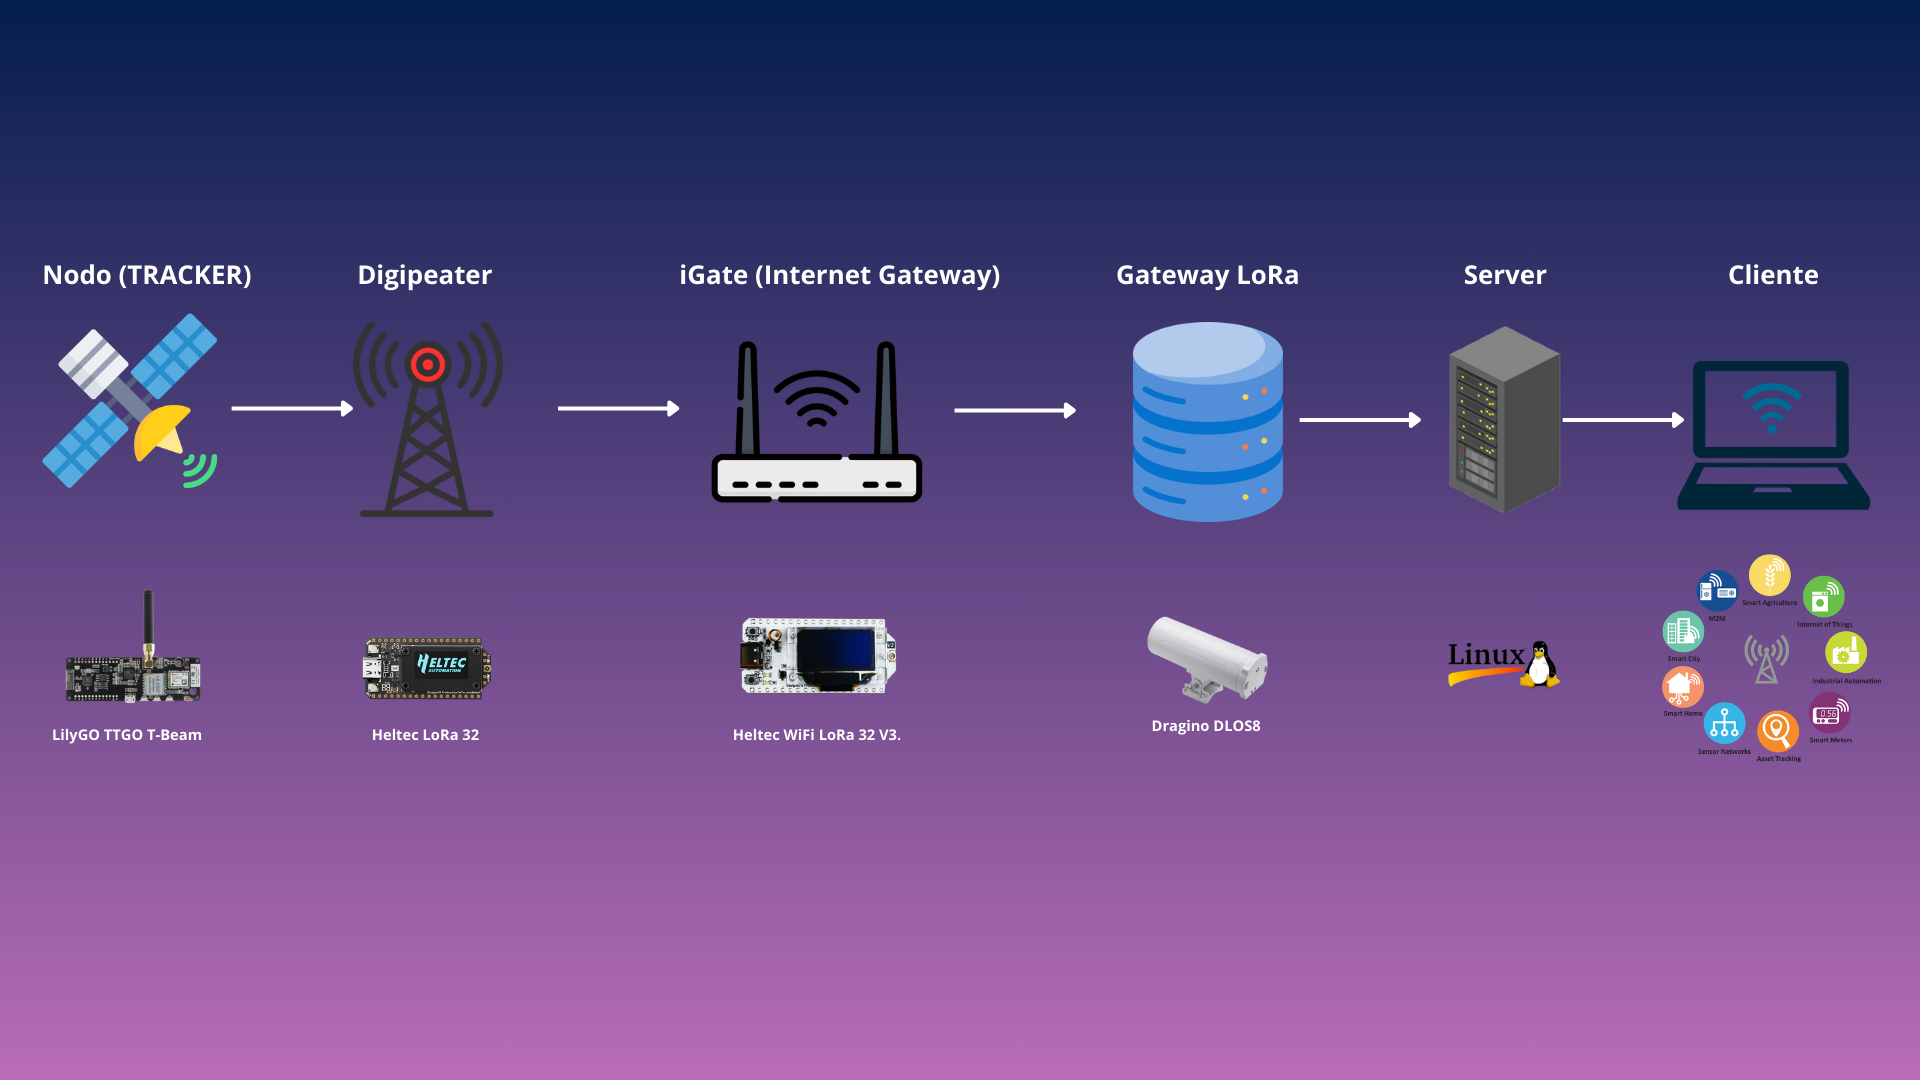
\includegraphics[width=\columnwidth]{Diagrama.png}
    \caption{Diagrama de red LoRa/APRS.}
    \label{fig:red_lora_aprs}
\end{figure}

\subsection{Capa Física y de Enlace (Modelo OSI)}
La modulación LoRa opera en la Capa 1 del modelo OSI. Para el establecimiento del enlace entre nodos e iGate, se consideran:

\subsubsection{Spreading Factor (SF)}
El \textit{Spreading Factor} determina la duración temporal de cada símbolo. A mayor SF, mayor sensibilidad y alcance, pero menor tasa de datos \cite{lorawan_state_2020}.

\subsubsection{Bandwidth (BW)}
El ancho de banda define el rango espectral del \textit{chirp} (125/250/500 kHz típicos). BW mayor aumenta tasa, pero reduce sensibilidad \cite{lorawan_state_2020}.

\subsubsection{Coding Rate (CR)}
La tasa de codificación implementa FEC, aumentando robustez a costa de mayor tiempo en aire \cite{lorawan_state_2020}.

\subsubsection{Sync Word}
Identificador de red; valores comunes \texttt{0x34} (público) y \texttt{0x12} (privado) \cite{sync_word_2025,semtech_faq_2024}.

\subsubsection{Adaptive Data Rate (ADR)}
El ADR ajusta SF y potencia según calidad del enlace para mejorar eficiencia espectral/energética \cite{adr_collision_2024}.

% ==============================
\section{Marco Regulatorio en Costa Rica}

\subsection{Cuadro Nacional de Atribución de Frecuencias (PNAF)}
El despliegue de sistemas de radiocomunicación en Costa Rica está regulado por el Estado para asegurar el uso eficiente del espectro y prevenir interferencias. El instrumento normativo central es el Plan Nacional de Atribución de Frecuencias (PNAF), actualizado mediante el Decreto Ejecutivo N\textsuperscript{o} 44010-MICITT, publicado en el Alcance N\textsuperscript{o} 99 a La Gaceta N\textsuperscript{o} 95 del 30 de mayo de 2023 \cite{pnaf_2023_micitt}. El PNAF adopta el marco del Reglamento de Radiocomunicaciones de la UIT y establece, para cada segmento del espectro, los servicios atribuidos (por ejemplo: fijo, móvil, aficionados) y notas nacionales aplicables.

\subsection{Bandas de Frecuencia Aplicables al Sistema LoRa/APRS}
El sistema LoRa/APRS puede operar, en Costa Rica, bajo dos escenarios regulatorios principales:

\subsubsection{Escenario A: Banda de radioaficionados (VHF 144--148 MHz)}
El PNAF atribuye los segmentos 144--146 MHz y 146--148 MHz al servicio de \textit{Aficionados} (y, donde aplica, aficionados por satélite), por lo que el uso de APRS clásico en 144.390 MHz se enmarca dentro del servicio de radioaficionados y requiere que la estación operadora cuente con habilitación/licencia correspondiente \cite{pnaf_2023_micitt,sutel_radioaficionados}.

\subsubsection{Escenario B: Bandas de uso libre para tecnologías digitales (902--940 MHz)}
El PNAF incorpora un \emph{Apéndice de bandas de uso libre}, definiendo condiciones técnicas y la obligatoriedad de homologación previa de equipos. En particular, el rango 902--940 MHz se incluye como banda de uso libre para tecnologías digitales, con límites máximos de potencia de salida y PIRE (EIRP) \cite{pnaf_2023_micitt}.

\subsection{Resumen normativo del PNAF para el proyecto}
La Tabla~\ref{tab:pnab_lora_aprs} resume los segmentos más relevantes para el sistema propuesto, separando la \emph{atribución de servicios} (Cuadro Nacional) y las \emph{condiciones de uso libre} (Apéndice V del PNAF).

\begin{table}[t]
\caption{Segmentos relevantes del PNAF para un sistema LoRa/APRS en Costa Rica}
\label{tab:pnab_lora_aprs}
\centering
\scriptsize
\setlength{\tabcolsep}{3pt}
\renewcommand{\arraystretch}{1.15}
\begin{tabularx}{\columnwidth}{@{}l l X l@{}}
\toprule
\textbf{Banda} & \textbf{Uso} & \textbf{Servicio en PNAF} & \textbf{Condición} \\
\midrule
144--148 & APRS VHF & Aficionados & Licencia \\
902--940 & LoRa/LPWAN & Uso libre  & Límites \\
\bottomrule
\end{tabularx}
\end{table}

\subsection{Clases de Emisión}
El PNAF utiliza la designación de la UIT para describir emisiones radioeléctricas. Una clase de emisión caracteriza (i) tipo de modulación de la portadora, (ii) naturaleza de la señal modulante y (iii) tipo de información transmitida. Para APRS clásico en VHF (AFSK 1200 bps) se utilizan designaciones del tipo \textbf{F2D}. Para LoRa (CSS) la clasificación depende del ancho de banda ocupado y del esquema de modulación digital, por lo que se reporta como una emisión digital en canal único (telemetría/datos), típicamente en familias \textbf{F1D/F7W} según el ancho de banda y parámetros de modulación \cite{itu_emissions}.

\subsection{P.I.R.E Permitida (EIRP) para bandas de uso libre}
El Apéndice V del PNAF define límites máximos por banda para equipos de baja potencia. En particular, para \textbf{902 a 940 MHz} se especifica \textbf{potencia máxima de salida de 24 dBm} y \textbf{PIRE máxima de 30 dBm}, lo cual condiciona el diseño de hardware (PA, antena y ganancia) y la configuración del enlace LoRa \cite{pnaf_2023_micitt}.

\subsection{Permisos y Trámites Requeridos}
La operación depende de la banda seleccionada:

\subsubsection{Bandas de uso libre (p.\ ej., 902--940 MHz)}
No requieren concesión individual; sin embargo, el PNAF establece que previo a la utilización de bandas de uso libre debe realizarse el procedimiento de \textbf{homologación} del equipo ante SUTEL \cite{pnaf_2023_micitt,sutel_homologacion_2018}. Este trámite verifica cumplimiento de límites técnicos (potencia, PIRE, máscaras espectrales y requisitos aplicables).

\subsubsection{Bandas de radioaficionados (p.\ ej., 144--148 MHz)}
Requieren \textbf{licencia/permiso de operación} del servicio de radioaficionados y cumplimiento de condiciones asociadas (indicativo, responsabilidades operativas y compatibilidad electromagnética) \cite{pnaf_2023_micitt,sutel_radioaficionados}.

\subsection{Mapa de Tiempos de Trámites Regulatorios}
Con el objetivo de evaluar la viabilidad administrativa del despliegue del sistema LoRa/APRS, se presenta un análisis comparativo de los trámites requeridos según la banda de operación seleccionada, conforme al PNAF y la normativa vigente \cite{pnaf_2023_micitt,sutel_homologacion_2018,sutel_radioaficionados}.

\subsubsection{Escenario A: Banda de Uso Libre (902--940 MHz)}
En este escenario no se requiere concesión individual del espectro; sin embargo, el PNAF establece la obligatoriedad de homologar previamente el equipo ante la Superintendencia de Telecomunicaciones (SUTEL).

\begin{table}[t]
\caption{Mapa de tiempos para operación en banda de uso libre (902--940 MHz)}
\label{tab:mapa_tiempos_uso_libre}
\centering
\scriptsize
\setlength{\tabcolsep}{3pt}
\renewcommand{\arraystretch}{1.15}
\begin{tabularx}{\columnwidth}{@{}l X l l@{}}
\toprule
\textbf{Instancia} & \textbf{Trámite} & \textbf{Tiempo} & \textbf{Resultado} \\
\midrule
SUTEL & Homologación de equipo (uso libre) & $\leq$10 días hábiles & Resolución \\
\bottomrule
\end{tabularx}
\end{table}

El proceso consiste en la presentación de documentación técnica del dispositivo (especificaciones, potencia de salida, certificaciones internacionales) a través de la plataforma oficial de homologación. Una vez aprobado, el equipo puede operar dentro de los límites técnicos establecidos (24 dBm potencia de salida y 30 dBm PIRE).

\subsubsection{Escenario B: Banda de Radioaficionados (144--148 MHz)}
En este caso se requiere licencia de radioaficionado y autorización de uso del espectro.

\begin{table}[t]
\caption{Mapa de tiempos para operación en banda de radioaficionados (144--148 MHz)}
\label{tab:mapa_tiempos_radioaficionados}
\centering
\scriptsize
\setlength{\tabcolsep}{3pt}
\renewcommand{\arraystretch}{1.15}
\begin{tabularx}{\columnwidth}{@{}l X l l@{}}
\toprule
\textbf{Instancia} & \textbf{Trámite} & \textbf{Tiempo} & \textbf{Resultado} \\
\midrule
SUTEL & Evaluación / criterio técnico & Variable & Dictamen \\
MICITT & Emisión de licencia / autorización & 3--6 meses (aprox.) & Licencia \\
\bottomrule
\end{tabularx}
\end{table}

El proceso incluye la acreditación como radioaficionado (según categoría), evaluación técnica y resolución ejecutiva. Debido a la intervención de múltiples instancias administrativas, el tiempo total del trámite es significativamente mayor que en el régimen de uso libre.

\subsubsection{Análisis Comparativo}
Desde el punto de vista administrativo y temporal, la operación en la banda 902--940 MHz bajo régimen de uso libre representa la alternativa más viable para un proyecto académico de duración semestral, debido a la simplicidad del trámite y su corto plazo de resolución.
% ==============================
\section{Conclusiones}

En el informe se realizó una investigación inicial sobre los fundamentos de los sistemas de comunicación APRS y la tecnología LoRa, analizando su funcionamiento, arquitectura de red y principales parámetros de operación. A partir de esta investigación, se identificó que la combinación de ambas tecnologías permite implementar sistemas de telemetría y monitoreo remoto con bajo consumo energético y gran alcance de comunicación.

Asimismo, se estudió la legislación costarricense relacionada con el uso del espectro radioeléctrico, particularmente el Plan Nacional de Atribución de Frecuencias (PNAF). Esto permitió identificar las bandas disponibles para la implementación del sistema propuesto, así como las restricciones técnicas asociadas a potencia de transmisión y P.I.R.E. permitida.

A partir de la arquitectura de red analizada, se determinó que el componente \textit{iGate} desempeña un papel fundamental dentro del sistema APRS, al actuar como puente entre la red de radio y la infraestructura de servidores en Internet.

% ==============================
\bibliographystyle{IEEEtran}
\bibliography{referencias}

\end{document}
